\documentclass[25pt,a1paper, portrait, colspace = 0.5cm, blockverticalspace = 5mm]{tikzposter}
\usepackage{blindtext}
\usepackage{comment}

\title{Steam Engines and Economic Development}
\author{Sebastian T. Braun, Richard Franke, Timur Öztürk*}
\date{\today}
\institute{University of Bayreuth}
\usetheme{Envelope}
\colorlet{notebgcolor}{orange}
\colorlet{noteframecolor}{orange}


\begin{document}

\maketitle[titlegraphictotitledistance=-1.5cm,titletoblockverticalspace=0.5cm]

\block{\Large Regional Industrialization in Germany: Patterns, Diffusion and Long-Term Effects}
{

\begin{itemize}
\item The project’s first objective is to construct a novel, plant-level dataset on the adoption of steam engines, one of the defining innovation of the First Industrial Revolution, \textbf{in Württemberg from 1840 onwards}. 
\item The dataset’s \textbf{primary sources are handwritten reports on newly installed steam engines}, published annually by Württemberg’s Ministry of the Interior.
\item The data have several advantages compared to previously used sources:
\begin{itemize}
\item First, \textbf{\emph{the data are available each year.}} In contrast, previous studies for Prussia and Germany (Banken, 1993; Rook, 1978) draw on data for specific census years.
\item Second, the data contain each\textbf{ \emph{steam engine’s exact location}} (parish, type of factory) and owner. Existing studies on the diffusion of steam in Germany (Banken, 1993) and England (Nuvolari et al., 2011) focus on the district or county level – and thus on a much higher level of aggregation. 
\item Third, the data contain a wealth of additional information on, for example, \textbf{\emph{the type and producer of each steam engine and its power, purpose and weight.}}
\end{itemize}
\end{itemize}
}


\note[
        targetoffsetx=14.6cm,
        targetoffsety=14cm, angle=20, rotate=25,width = 0.25\linewidth
        ]
        {\small \textbf{\,\,\,\,\,\emph{timurozturk.org/TUC22} for more! }}

\begin{columns}
    \column{0.45}
    \block{Visualization}
    {
        \begin{tikzfigure}
	\vspace{-1.2cm}
            \includegraphics[height=280mm]{FinalBorders.jpg}
        \end{tikzfigure}
    }
    \column{0.55}
    \block{How do we do it?}
	{
		We use \textbf{Transkribus} for converting our data from 19th century German handwriting to an Excel format. Instead of training our own data, we use readily available models provided by the program. Then using \textbf{Python} and \textbf{pandas} we finalize our dataset. \\ \\ \vspace{-0.7cm}\hspace{-5mm} 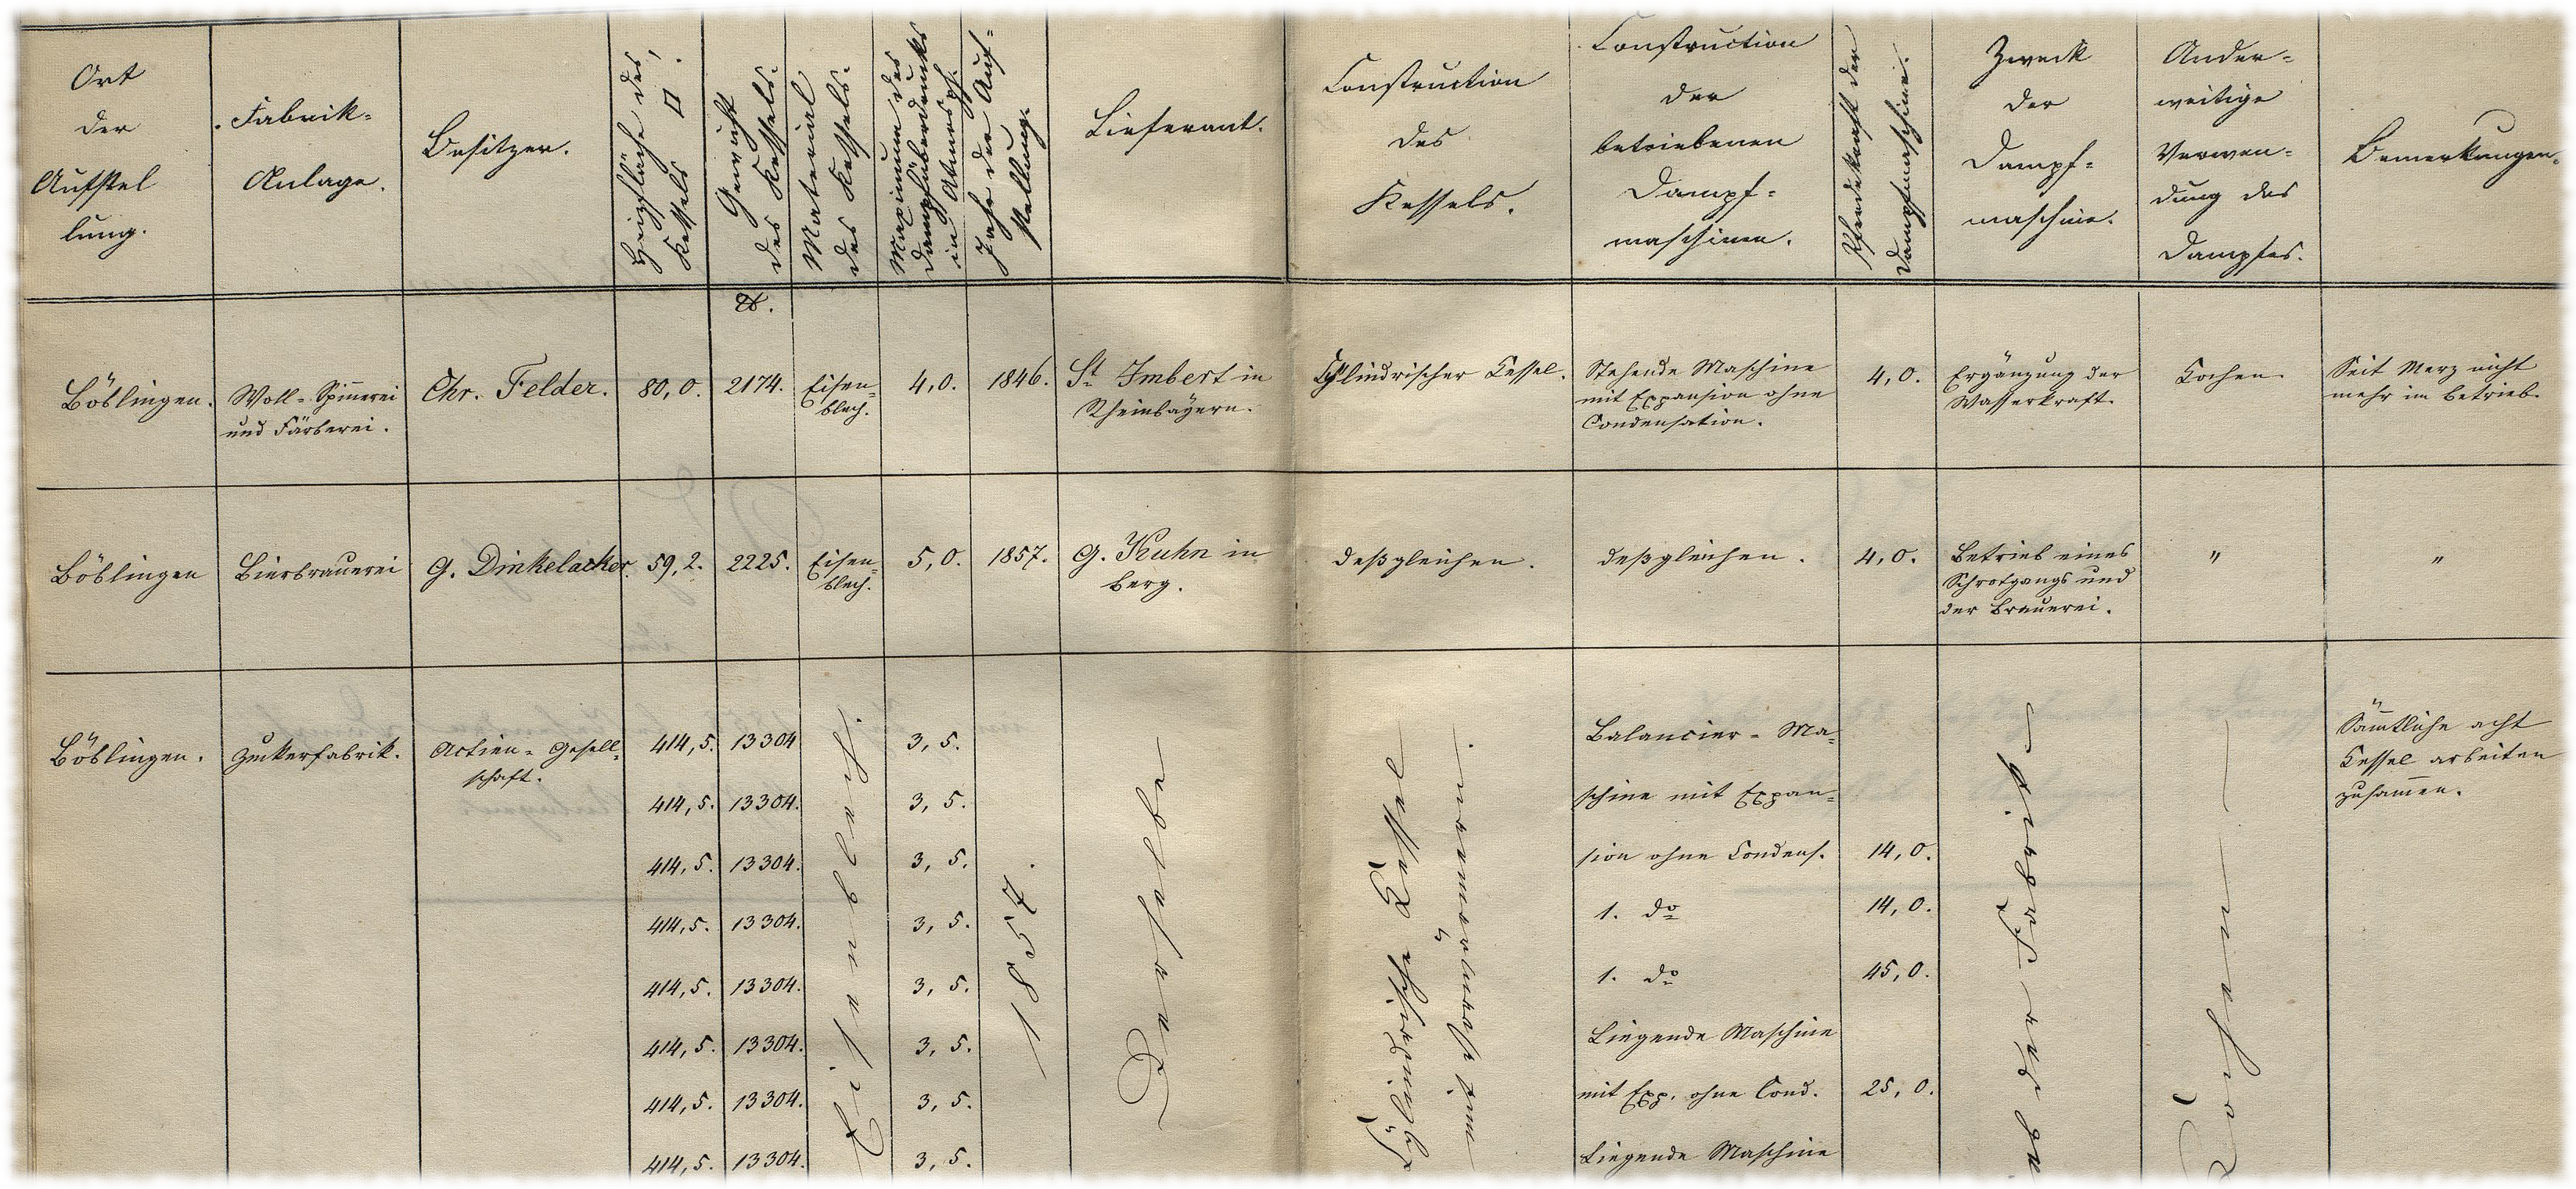
\includegraphics[height=13.2cm]{Steam.png}	}
\block{}{\textbf{Follow us!} The project is new and there is so much to share! \vspace{5mm}

\textbf{Timur Öztürk} \hspace{1cm} \textbf{Prof. Sebastian Braun} \hspace{1cm} \textbf{VWL VII} \vspace{5mm}

\hspace{1.28cm} \includegraphics[height=3cm]{ozturk.png} \hspace{6.5cm} \includegraphics[height=3cm]{braun.png} \hspace{5.5cm} \includegraphics[height=3cm]{vwl7.png} \vspace{8mm}}
\end{columns}

\begin{columns}

    \column{1}
    \block{Research Aim}{ Why does new technology spread only slowly across firms? Our project will shed new light on barriers and pathways to technology adoption for a fascinating historical case: \textbf{the diffusion of steam technology in Württemberg.} Not only was the steam engine one of the key technologies during Germany’s industrialization, but Württemberg’s firms were also late in adopting the new technology. Potential reasons for Württemberg’s late adoption are the lack of domestic coal and the poor transport infrastructure. To the best of our knowledge, the analysis will be the first to provide a plant-level perspective on the adoption of steam
\begin{itemize}
\item Did larger or export-oriented plants drive the \textbf{adoption of steam in Württemberg}?
\item Did early adopters generate \textbf{spill-over effects}?
\item Did the\textbf{ local transport infrastructure} (roads, navigable waterways and railways) affect plants’ adoption decisions?
\end{itemize}
 Financial support from the Deutsche Forschungsgemeinschaft (DFG,471335227) is gratefully acknowledged.}
\end{columns}
\end{document}